% This is main.tex, a sample paper demonstrating the use of the
% LLNCS macro package for Springer Computer Science proceedings;
% Version 2.20 of 2017/10/04
% 
\documentclass[runningheads]{llncs}
\usepackage[a4paper,left=3cm,right=3cm,top=4cm,bottom=4cm,bindingoffset=5mm]{geometry}
%
% ---- Packages ----
%
\usepackage{graphicx} % enhanced support for graphics
\usepackage{url} % add macros for handling URLs in text
\usepackage[nohyperlinks,nolist]{acronym} % abbreviation utilities
\usepackage{listings}
% TODO: add more packages below if necessary
%
% ---- Acronyms ----
%
\begin{acronym}
\acro{rq}[RQ]{Research Question}
% TODO: define more acronyms here
\end{acronym}
%
% ---- Begin Document ----
%
\begin{document}
%
\title{Similarity classification of HTML with Large Language Models}
%
%\titlerunning{Abbreviated paper title}
% If the paper title is too long for the running head, you can set
% an abbreviated paper title here
%
% ---- Author Information ----
%
\author{Timo Kühne}
\institute{Seminar: Software Quality\\
Advisor: Andrea Stocco\\
Technical University of Munich\\
\email{timo.kuehne@tum.de}}
%
\maketitle % typeset the header of the contribution
%
% ---- Abstract ----
%
\begin{abstract}
The abstract should briefly summarize the contents of the paper in
15--250 words.

\keywords{First keyword  \and Second keyword \and Another keyword.}
\end{abstract}
%
% ---- Text Parts ----
%
\section{Introduction}
\label{sec:intro}
The titles of theses at TUM have to follow specific guidelines.
Find more information under this link:
\url{https://www.tum.de/fileadmin/w00bfo/www/Studium/Dokumente/Pruefungsangelegenheiten/The_Use_of_English_in_Thesis_Titles_at_TUM.pdf}

\subsection{Motivation}
\label{subsec:motivation}

Please note that the first paragraph of a section or subsection is not indented.
The first paragraph that follows a table, figure, equation etc.
does not need an indent, either.\footnote{Here is a sample footnote with a URL: \url{http://google.com}}

Subsequent paragraphs, however, are indented.

\subsubsection{Sample Heading (Third Level)} Only two levels of
headings should be numbered.
Lower level headings remain unnumbered; they are formatted as run-in headings.

\paragraph{Sample Heading (Fourth Level)}
The contribution should contain no more than four levels of headings. 
Table~\ref{tab:tab1} gives a summary of different text styles.

\begin{table}
\caption{Table captions should be placed above the
tables.}\label{tab:tab1}
\centering
\begin{tabular}{|l|l|l|}
\hline
First col &  Second col & Third col\\
\hline
Normal & \textbf{Bold} & \textit{Italique}\\
\texttt{Typewriter} & \textsc{small caps} & \underline{underline}\\
\hline
\end{tabular}
\end{table}


\noindent Displayed equations are centered and set on a separate
line.
\begin{equation}
x + y = z\label{eq:equation}
\end{equation}
Please try to avoid rasterized images for line-art diagrams and schemas. 
Whenever possible, use vector graphics instead (see Fig.~\ref{fig:fig1}).

\begin{figure}
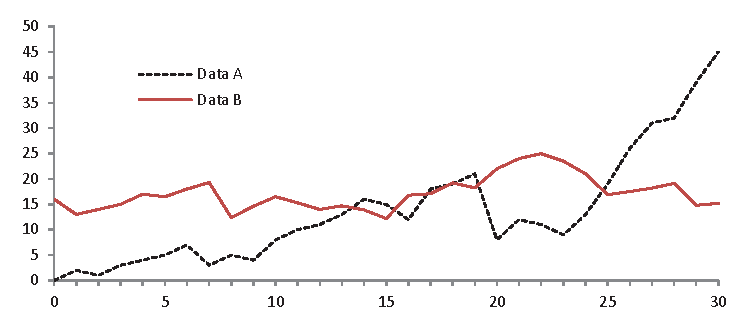
\includegraphics[width=\textwidth]{figures/fig1}
\caption{A figure caption is always placed below the illustration.
Please note that short captions are centered, while long ones are justified by the macro package automatically. The text within graphics should be readable in the printed version.} 
\label{fig:fig1}
\end{figure}

\begin{theorem}
This is a sample theorem. 
The run-in heading is set in bold, while the following text appears in italics. 
Definitions, lemmas, propositions, and corollaries are styled the same way.
\end{theorem}
%
% the environments 'definition', 'lemma', 'proposition', 'corollary',
% 'remark', and 'example' are defined in the LLNCS documentclass as well.
%
\begin{proof}
Proofs, examples, and remarks have the initial word in italics, while the following text appears in normal font.
\end{proof}
For citations of references, we prefer the use of square brackets and consecutive numbers. 
Citations using labels or the author/year convention are also acceptable. 
The following bibliography provides a sample reference list with entries for journal articles~\cite{Stol2016}, a book~\cite{Myers2012}, conference proceedings~\cite{Harrold1988}, and a web site~\cite{Schaffer2018}.

\subsection{Abbreviations}
\label{subsec:abbrev}

To use acronyms in the document, simple declare them in the main.tex file and use them later.
For example, you might want to define \acp{rq}, which will then be always abbreviated as \ac{rq} for singular or \acp{rq} for plural.

List are also really easy to create:

\begin{itemize}
  \item One entry in the list
  \item Another entry in the list
\end{itemize}

\begin{enumerate}
  \item The labels consists of sequential numbers.
  \item The numbers starts at 1 with every call to the enumerate environment.
\end{enumerate}

\subsection{Code Listings}
\label{subsec:code}

Listings can either be created inside the text or imported:\footnote{See \url{https://www.overleaf.com/learn/latex/Code_listing} for a complete example.}
\begin{lstlisting}[language=C,label={lst:lstlisting}]
int main(int argc, char* argv[]) {
  return 0;
}
\end{lstlisting}
\section{Conclusion}
    \label{sec:conclusion}
    
    This paper introduced GeminiScan, a novel LLM-based approach to near-duplicate detection in web testing. By combining a small-scale LLM for efficient inference with a large-scale LLM for prompt optimization, our method addresses challenges in semantic understanding and generalization.
    
    Evaluation of the Addressbook and PetClinic applications from the Yandrapally et al. 2020 dataset demonstrated competitive performance, with F1 scores of 0.87 and 0.78, respectively. Furthermore, GeminiScan outperforms traditional methods like RTED and approaches the effectiveness of state-of-the-art techniques such as WebEmbed and FragGen. Key strengths include strong performance in identifying distinct pages, effective near-duplicate detection, and a low false positive rate. While computational requirements present a challenge, our automated feedback loop for prompt optimization showcases the potential for continuous improvement. Future work could focus on expanding the evaluation to more diverse web applications, reducing computational requirements, and further improving classification accuracy.
    
    GeminiScan represents a significant step in applying advanced \ac{nlp} techniques to web testing, opening new opportunities for research in software quality assurance. As LLM technology rapidly advances, we anticipate further improvements in the efficiency and effectiveness of near-duplicate detection in web testing. This could possibly lead to the replacement of manual test creation in the future.
%
% ---- Appendix ----
%
\appendix
\section{Appendix}
\label{sec:appendix}

Anything additional goes here \dots
%
% ---- Bibliography ----
%
\bibliographystyle{splncs04}
\bibliography{library.bib}
%
\end{document}
